\documentclass[10pt]{beamer}

\usepackage[french]{babel}
\usepackage[utf8]{inputenc}
\usepackage[T1]{fontenc}
\usepackage{lmodern}
\usepackage{tikz}
\usetheme{Warsaw}

\title[IA et conduite autonome]{Utilisation de l'intelligence artificielle dans la manœuvre autonome de bateau}
\author{Maxime CAUTRÈS}
\institute{Lycée Blaise Pascal}
\date{01/03/2020}


\AtBeginSection[]
{
  \begin{frame}
  \frametitle{Sommaire}
  \tableofcontents[currentsection, hideothersubsections, pausesubsections]
  \end{frame} 
}

\logo{
\includegraphics[height=10mm]{logo_limos_coul_def.png}}


\begin{document}

\begin{frame}
  \titlepage
\end{frame}



\section{Introduction}

\begin{frame}{allowframebreaks}{\label{deb}}
  
  \frametitle{Mise en contexte}
 
  \begin{figure}
    \begin{center}
      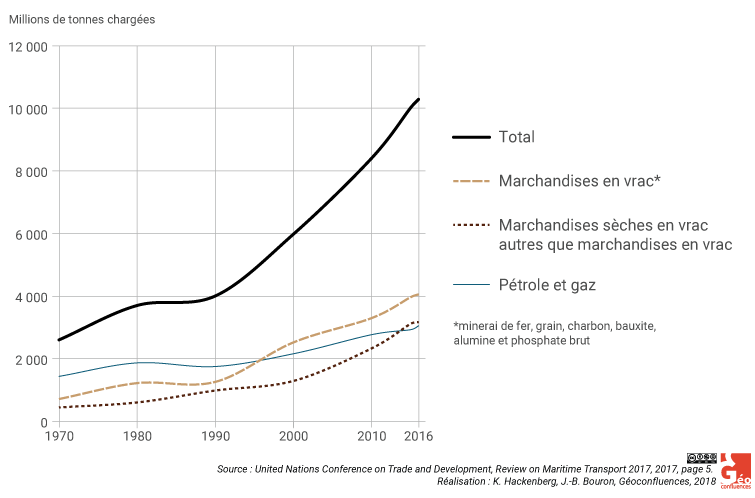
\includegraphics[height=50mm]{courbe_evo_bateau.png}
      \caption{La croissance du commerce maritime international (en millions de tonnes chargées)}
    \end{center}
  \end{figure}
  
  
\end{frame}

\section{Le cerveaux}

\begin{frame}{allowframebreaks}[\label{2}]
  \frametitle{un cerveau pas tres malin}
  bonsoir a tous personnelement
  je suis entrain de passer un bon momeny
 
  \hyperlink{deb}{aller au laber 1}
\end{frame}

\end{document}

\begin{frame}
  \frametitle{Sommaire}
  \tableofcontents
\end{frame}

http://geoconfluences.ens-lyon.fr/informations-scientifiques/dossiers-regionaux/territoires-europeens-regions-etats-union/rte-t/port-anvers

c'est le lien de l'image de l'intro
